%==========================================================
% PART 7: the live watch (Phase 7).
%==========================================================
\clearpage
\begin{center}
\begin{minipage}{0.86\textwidth}
\small
\textbf{Part 7: any city, now.} Part 6 replays two storms that already happened. A warning system has to work on the
storm that is happening tonight, in a town nobody prepared in advance. This part describes the \emph{live watch}: you
type the name of a city, the system sets itself up there in a few minutes, and from then on it follows the rain and
the flood model every five minutes, and sounds the alarm on screen and by email. Same rules as before: every word
explained, real numbers only, the simulation clearly labelled.
\end{minipage}
\end{center}

\begin{careful}
\textbf{What is live and what is simulated.} The weather, the terrain, the land cover, the soil and the tower positions
we can find are real and current. No operator shares its link signals with us, so by default the links between the
towers and their signals are \emph{simulated} from the live weather, and the AI reads the rain back from them. This shows
the whole chain running on any city, live; it does not measure how accurate it would be there. When an operator
connects its real link data (Section~\ref{sec:p7_modes}), the same chain runs on real signals.
\end{careful}

%==========================================================
\section{What the user does}
\label{sec:p7_user}
%==========================================================
\begin{enumerate}[itemsep=0.25em]
\item \textbf{Type a city.} The page asks an open map service (OpenStreetMap's Nominatim) for places with that name and
shows a short list, because a name alone is ambiguous (``Constantine'' is also a district, ``Tunis'' also a country).
Picking one flies the map there.
\item \textbf{Choose where the signals come from:} \emph{Simulation} or \emph{My own data}
(Section~\ref{sec:p7_modes}).
\item \textbf{Wait for the set-up.} A list on the page ticks off each step (Section~\ref{sec:p7_setup}). It takes a few
minutes the first time; everything is kept, so a restart of the server picks up where it stopped.
\item \textbf{Watch.} The screen shows the towers and links coloured by the rain they see, the rain map, the flood water,
the alert level, the last 24 hours as two small charts, and a log of every change of level (Figure~\ref{fig:p7_watch}).
\item \textbf{Get the alarm.} When the level reaches \emph{flood warning} or \emph{flooding}, an email goes out, and
another when it is over. The first visit to the page asks where alarms should go.
\end{enumerate}

\begin{figure}[h]
\centering
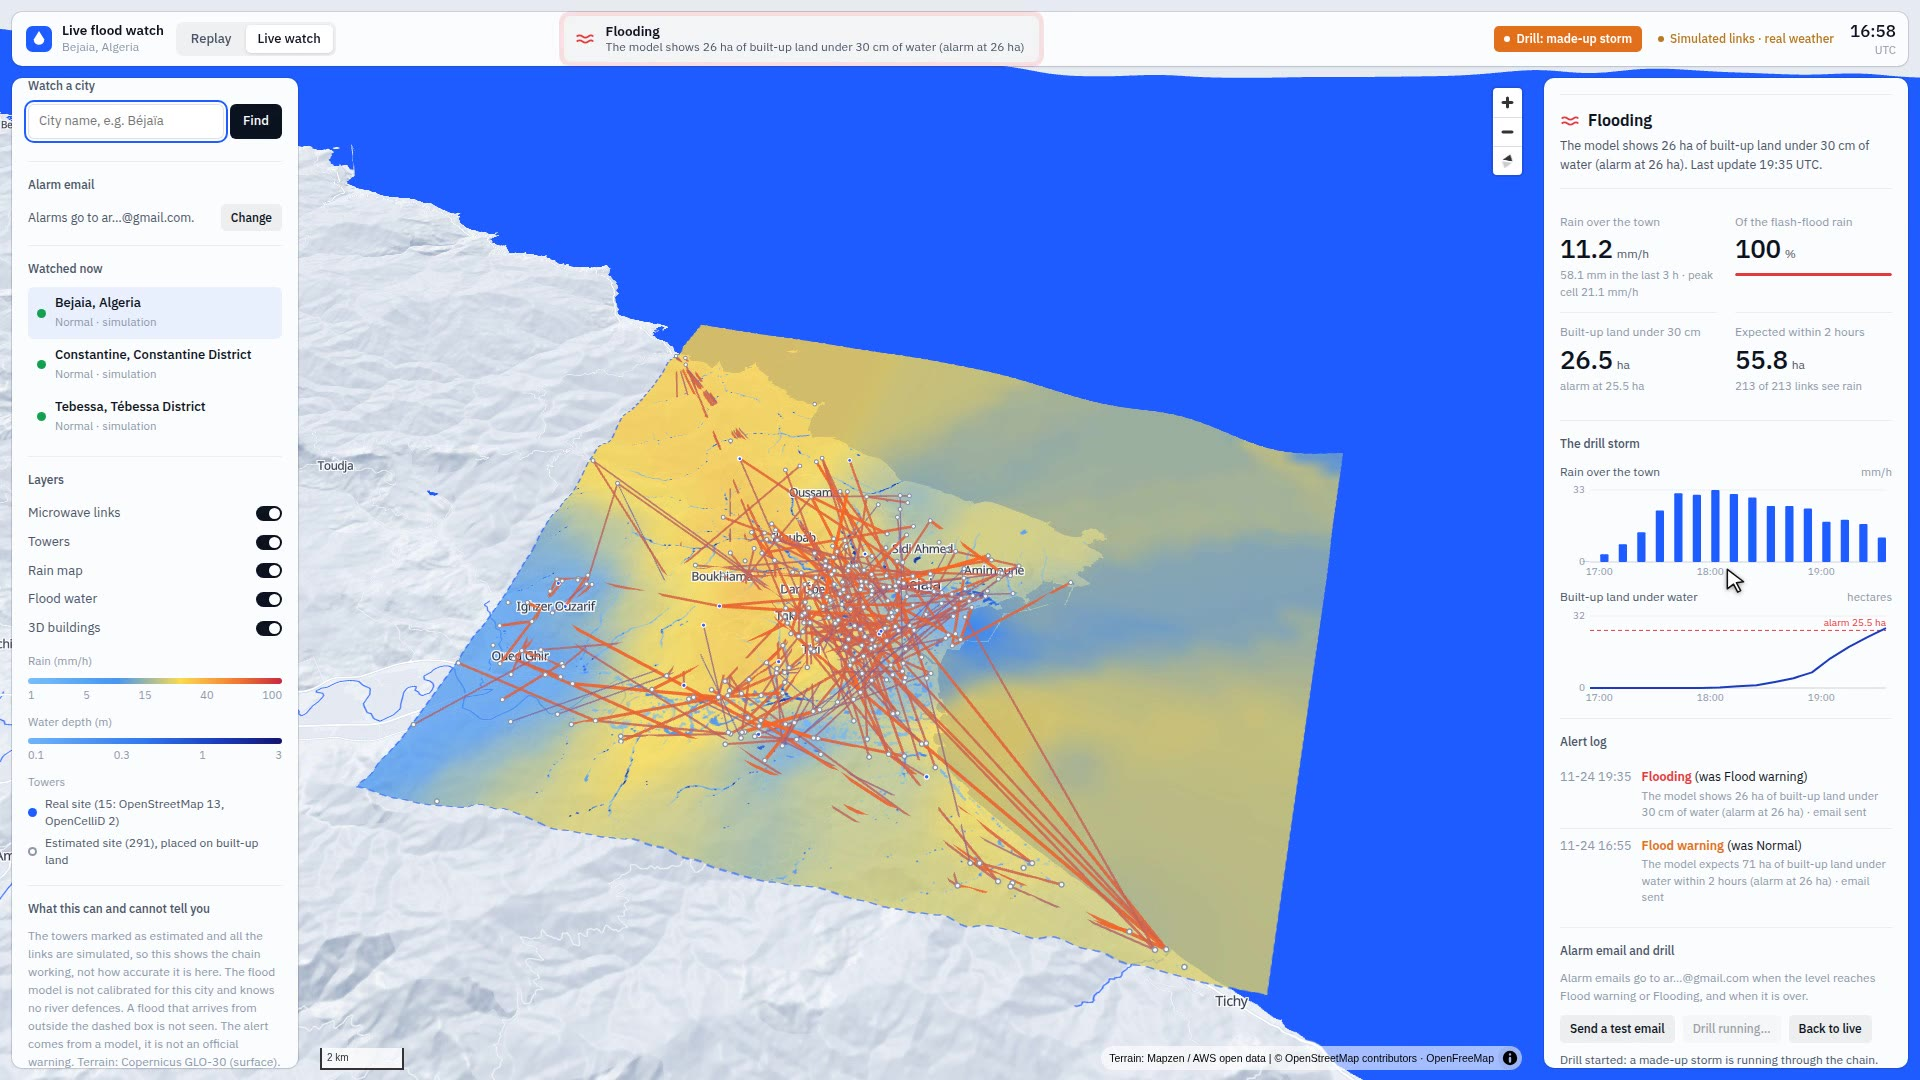
\includegraphics[width=\textwidth]{fig_p7_watch.jpg}
\caption{The live watch on Béjaïa during a drill (Section~\ref{sec:p7_drill}), at the moment the town floods. Left: the
watched cities, the alarm email and the layers. Centre: the city in 3D, with the towers, the links (orange: wet) and the
rain map over the watched box. Right: the alert level, the figures of the moment, the drill storm and the flooded
built-up land crossing the red alarm line, and the alert log, where both changes of level show ``email sent''. The
orange badge at the top marks the drill.}
\label{fig:p7_watch}
\end{figure}

%==========================================================
\section{Setting up a city nobody prepared}
\label{sec:p7_setup}
%==========================================================
For Algiers and Ghardaïa (Parts 4 to 6) we prepared each piece by hand. The live watch does the same for any place,
alone, from free worldwide sources. The watched box is about 18 by 18\,km around the centre of the town (at most
30 by 30\,km, so one computer keeps up).

\textbf{1. The ground.} The same three maps as the flood model of Part~5, cut to the box: the Copernicus 30\,m terrain,
the ESA WorldCover land cover (built-up, trees, crops, water...) and the soil type (from NASA's HYSOGs map, when a free
Earthdata key is set; otherwise an average soil, and the page says so).

\textbf{2. The towers.} No single source covers the world. OpenCelliD, our source for Algiers, has thousands of sites
there, but its free service allows only a small number of requests a day; OpenStreetMap is free but has few masts
(145 in Algiers, against 4,092 sites in OpenCelliD). So the watch uses three tiers:
\begin{itemize}[itemsep=0.1em]
\item OpenCelliD sites already saved for the area, if any;
\item mast and antenna positions from OpenStreetMap;
\item \emph{estimated} sites, to fill the gap up to a normal city density, placed on built-up land with a typical spacing
per operator.
\end{itemize}
Every tower is marked real or estimated, drawn differently on the map (blue: real; white: estimated), and counted on
the page. Béjaïa has 15 real sites (13 from OpenStreetMap, 2 from OpenCelliD) and 291 estimated ones.

\textbf{3. The links.} Built per operator between nearby towers, with the method of Part~4 (Section~\ref{sec:p4_network}):
operators do not share their networks, so a link always joins two towers of the same operator. Béjaïa: 213 links.

\textbf{4. The rain that floods the town.} As in Part~5, the flood model is run on made-up storms of growing size
(15, 25, 40, 60, 90, 130 and 180\,mm), falling evenly over one hour and over three hours, until the built-up land under
30\,cm of water reaches the alarm size. For Béjaïa: \textbf{46\,mm in one hour} or \textbf{58\,mm in three hours}, and
an alarm size of 25.5\,ha of built-up land.

%==========================================================
\section{The three ways to get the signals}
\label{sec:p7_modes}
%==========================================================
\begin{description}[leftmargin=0pt,itemsep=0.3em]
\item[A known live source.] A list in the project (\texttt{configs/live\_sources.yaml}) says which places have an
operator feed. It is empty today, because no operator publishes link data. It is the place an agreement with an
operator would be registered; the city would then be watched on real signals without any question asked.
\item[My own data.] An operator, or anyone with link records, delivers two tables in one simple standard format: the
links (an identifier, the two ends, the frequency, the polarisation) and the readings (time in UTC, link, received and
sent level in dBm), at least every 15 minutes. If their system already serves these tables at two web addresses, that
is all. If it stores them differently, a small \emph{adapter} file of two functions translates them; a template comes
with the project. Before the watch starts, the page reads the data and lists, in plain words, anything that does not
fit (a missing column, a wrong unit, times not in UTC, a link without readings).
\item[Simulation.] The default. The live rain comes from a weather service (Open-Meteo: free, worldwide, every 15
minutes, radar-fed where a country has radar). It is sharpened to 500\,m and 1 minute as in Part~4, pushed through the
simulated links with the same physics (the ITU formula, wet antennas, real dry-day noise), and the AI reads it back.
\end{description}

\begin{careful}
\textbf{Safety.} Adapter code is never sent through the web page: it is a file placed on the server by whoever runs it,
and the page only lists the adapters that are installed. Otherwise anyone who can open the page could run programs on
the server.
\end{careful}

%==========================================================
\section{Every five minutes}
\label{sec:p7_cycle}
%==========================================================
Once a city is set up, the watch repeats the same steps every five minutes:
\begin{enumerate}[itemsep=0.2em]
\item read the new signal levels of every link (or simulate them);
\item the AI turns each link's signal into rain along that link (Part~2);
\item the links' rain becomes a rain map of the box (Part~3);
\item the flood model moves the water forward five minutes, keeping the water, the flows and the soil wetness of the
step before (Part~5);
\item a \emph{look-ahead}: a copy of the flood model runs two hours ahead on the rain the weather service expects;
\item the alert level is set, and an email goes out if it rose to flood warning or flooding.
\end{enumerate}

\textbf{The four levels} are the same as in the control room, with one change: \emph{flood warning} now comes from the
look-ahead.
\begin{itemize}[itemsep=0.1em]
\item \textbf{normal};
\item \textbf{watch}: the rain of the last hours reaches half of the rain that floods the town, or the look-ahead shows
half of the alarm size;
\item \textbf{flood warning}: the look-ahead shows the town flooding within two hours;
\item \textbf{flooding}: the model shows the town flooding now (built-up land under 30\,cm at the alarm size).
\end{itemize}
A level rises at once but only falls after three calmer readings in a row (15 minutes), so the alarm does not flicker
on and off while a storm hesitates.

\textbf{How fast.} On the project computer's graphics card, a whole five-minute cycle for Béjaïa takes about 5 seconds.
On an ordinary processor (8 cores, no graphics card) the whole cycle, look-ahead included, takes about 25 seconds, so the
watch still keeps up comfortably. The slow part without a graphics card is the set-up of a \emph{new} city: finding the rain
that floods the town needs up to 14 flood runs of several hours of storm each. That takes minutes on a graphics card but
can take hours on a processor alone, especially for a large city. For that reason Béjaïa, Constantine and Tébessa come
already set up with the project: on a new computer they are watched within about two minutes.

%==========================================================
\section{Showing the alarm on a dry day: the drill}
\label{sec:p7_drill}
%==========================================================
Real flash floods are rare, so a judge, a mayor or a forecaster will usually see the watch on a calm day. The
\emph{drill} button runs a made-up storm through exactly the same chain: 2.2 times the three-hour rain that floods the
town (about 127\,mm in three hours for Béjaïa), falling over the watched box, read through the simulated links by the
AI, mapped and run through the flood model, four hours of storm in about two minutes on a graphics card (about 11 on 8 processor cores). On Béjaïa (drill of
24~November 2026) the look-ahead sees the town flooding from the first step, so the level goes straight from
\emph{normal} to \emph{flood warning}. The town floods 2\,h~40\,min of storm time later, when 26\,ha of built-up land
are under 30\,cm of water (the alarm size is 25.5\,ha); by the end of the drill it is 40\,ha. Each change sent its
email. The warning time is long here because a drill's forecast is perfect: the look-ahead knows the made-up storm in
advance. With a real forecast it will be shorter. The drill stops after four hours, while the town is still flooded,
so it shows the rise of the alarm but not the all-clear.

A drill never touches the live watch, which carries on underneath. It is labelled DRILL on every screen and in the
subject and first line of every email, so it cannot be mistaken for a real alarm.

%==========================================================
\section{The alarm email}
\label{sec:p7_email}
%==========================================================
One email per rise to \emph{flood warning} or \emph{flooding}, and an all-clear when the level is back to normal; never
one per cycle. It gives the city, the time, the level, the reason in one sentence (for example ``The model shows 32\,ha
of built-up land under 30\,cm of water, alarm at 26\,ha''), a link to the watch page, and the line \emph{simulated
links} or \emph{DRILL} when that applies.

The first time the page is opened it asks where alarms should go and which account sends them; a Gmail address with an
\emph{app password} (a password Google makes for one program, which can only send mail) is enough. A test button sends
one email to check it arrives. The settings stay on the server, the password is never shown again, and once an address
is set, only someone at the server's own computer can change it (in the Docker version anyone who can open the page can,
which is why the setup guide keeps that page on the computer itself). Without a sending account the emails are kept as
files on the server, so nothing is lost.

%==========================================================
\section{What it can and cannot tell you}
\label{sec:p7_limits}
%==========================================================
The page lists these limits next to the map:
\begin{itemize}[itemsep=0.2em]
\item \textbf{In simulation, it shows the chain working, not its accuracy.} Measuring accuracy needs real link signals
and rain gauges in that city, as we had in Sweden, Italy and the Netherlands.
\item \textbf{The flood model is not calibrated for the new city.} It has no storm drains and no river defences, and
uses an average soil when the soil map is not available.
\item \textbf{Floods from outside the box are missed.} A flood that starts far upstream, like Ghardaïa's
(Part~5), arrives from outside the watched box. The set-up warns when the rivers entering the box drain a large area
outside it.
\item \textbf{The AI reads heavy rain about 10\% low}, so the alarm can come a little late. We tried a fixed correction,
fitted on the training months and scored on a month it had never seen: it improved rain overall (bias $-7\%$ to $-2\%$)
but not the heavy hours that decide the alarm ($-10\%$ to $-12\%$), so it is not used. The real fix is to retrain with
more weight on heavy rain. The standard method of Part~1 is not used live at all: it needs 30 minutes of future signal.
\item \textbf{It is a demonstration, not an official warning.} An official service needs the operators' data, the
national weather service, and a pilot.
\end{itemize}

%==========================================================
\section{The choices, in one table}
\label{sec:p7_choices}
%==========================================================
\begin{center}\footnotesize\setlength{\tabcolsep}{4pt}
\begin{tabular}{>{\raggedright\arraybackslash}p{2.8cm}>{\raggedright\arraybackslash}p{3.6cm}>{\raggedright\arraybackslash}p{6.9cm}}
\toprule
Choice & Value & Why\\
\midrule
Place search & OpenStreetMap Nominatim & free and worldwide; returns a list, because a name alone is ambiguous\\
Watched box & about 18\,km, at most 30\,km & covers a town and its slopes; one computer keeps up\\
Towers & OpenCelliD, OpenStreetMap, then estimated & no single free source covers the world; every tower marked real or
estimated\\
Live rain & Open-Meteo & free, no key, worldwide, 15-minute steps, past hours and the next hours\\
Rain reader & the AI only & the standard method needs 30 minutes of future signal\\
Cycle & every 5 minutes & the step of the operators' signal logs and of Part~5's alarm\\
Warning & a 2-hour look-ahead & long enough to act, short enough for the forecast rain to mean something\\
Falling levels & after 3 calmer readings & no flickering alarm\\
Operator data & one standard format + small adapters & the operator keeps its systems; we read one format\\
Email & standard mail, settings on the server & works with any mail account; nothing secret in the code\\
\bottomrule
\end{tabular}
\end{center}

\textbf{How to open it.} Start the server with \texttt{python scripts/serve\_site.py} (or with Docker, see the setup guide
in the repository) and open \texttt{/watch/}. The hosted copy of the site has the replays but not the live watch, which
needs that server.
